% Chapter Template

\chapter{Hardware Sequential Implementation of the FM-Index} % Main chapter title

\label{Chapter3} % Change X to a consecutive number; for referencing this chapter elsewhere, use \ref{ChapterX}			
The main scope of this thesis is to implement the aforementioned algorithm on a specific \textsl{FPGA} board, with all the reference data stored in a memory accessible via bus interface. This chapter will aim to describe a first implementation of this algorithm that could be duplicated on one board and used in parallel.

\section{Conception}

%A first, sequential, model is presented in the Figures \ref{fig:seqschema} and \ref{fig:fsm}.\\
\begin{figure}[H]
    \centering
    \hspace*{-25mm}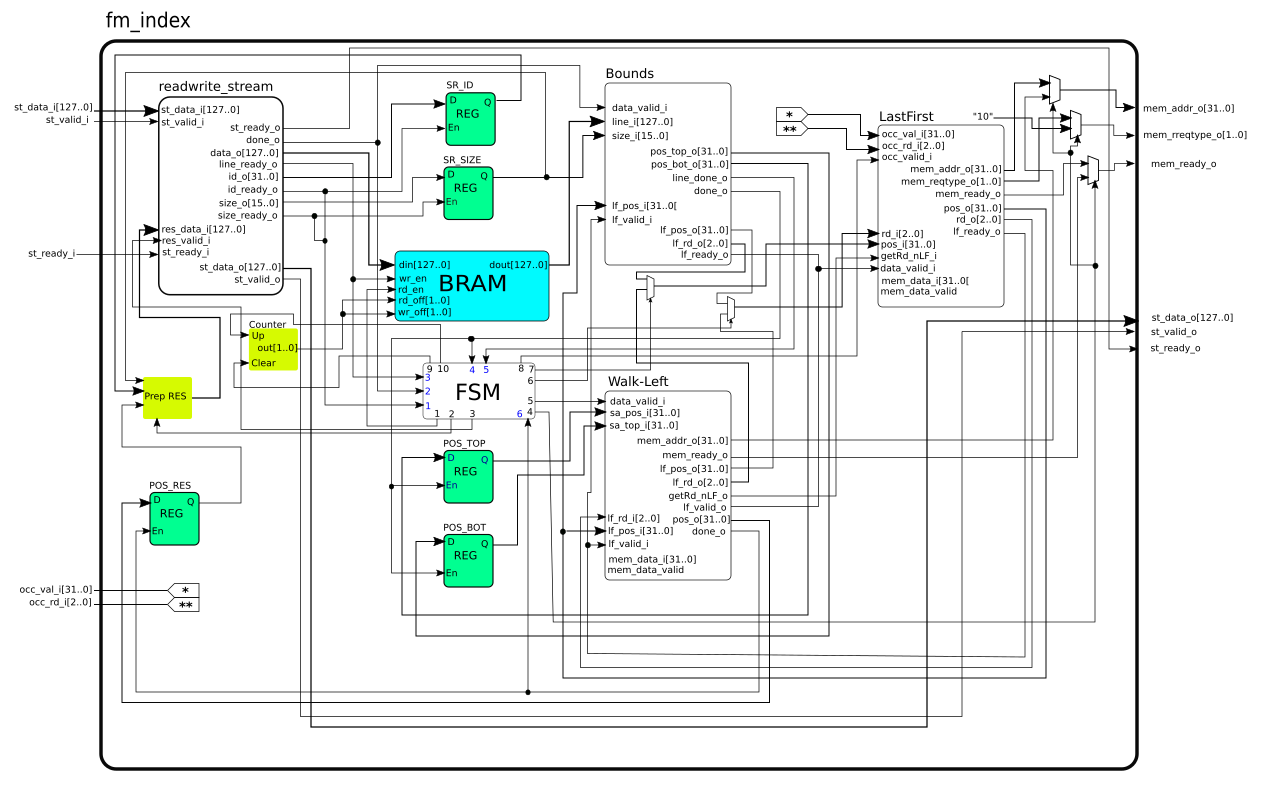
\includegraphics[scale = 0.45]{Figures/fmindex_top.png}
    \caption{Schema bloc of the FM-Index Top-Level}
    \label{fig:seqschema}
\end{figure}

Figures \ref{fig:seqschema} illustrate the hierarchy of the different blocks and element composing the \textsl{FM-Index}. \\

The details of the main FSM are described in Figure \ref{fig:fsm}, the different blocks are described in Section 3.1.2. Note that there are two different data input : one that is used to receive actual sequences to map onto the reference, the other is used to configure the \textsl{Occ} array, used in the LastFirst Mapping.

\subsection{FM-Index Global FSM}

This section illustrates the internal functioning of the \textsl{FM-Index} bloc, which is a hierarchical FSM, divided in 4 main steps as described below and illustrated in Figure \ref{fig:fsm}.
\begin{description}
\item [Read Sequence -] This loop is used to consume data from the \textsl{PCI Express Interface} in order to load a short read to align in the reference text along with an ID value associated to it.
\item [Bounds] - This loop scans the input sequence $q$ and, at each iteration, queries the \textsl{HMC} memory to update $top$ and $bot$. Note that is corresponds to Algorithm \ref{alg:match}.
\item [Walk Left] - This loop corresponds to Algorithm \ref{alg:WL}. It is only reached when the precedent loop ends up with a valid range for $q$ in the suffix array, i.e. $q$ exists in the reference text. Then again, at each iteration, the HMC is queried to update the index.
\item [Send Result] - This last part of the FSM sends back the results, whether $q$ was found or not, back to the result FIFO in the \textsl{PCI Express Interface}. This result contains the position (special value if not found), along with the ID corresponding to the query, stored in the \textsl{Read Sequence} step.
\end{description}
\begin{figure}[H]
 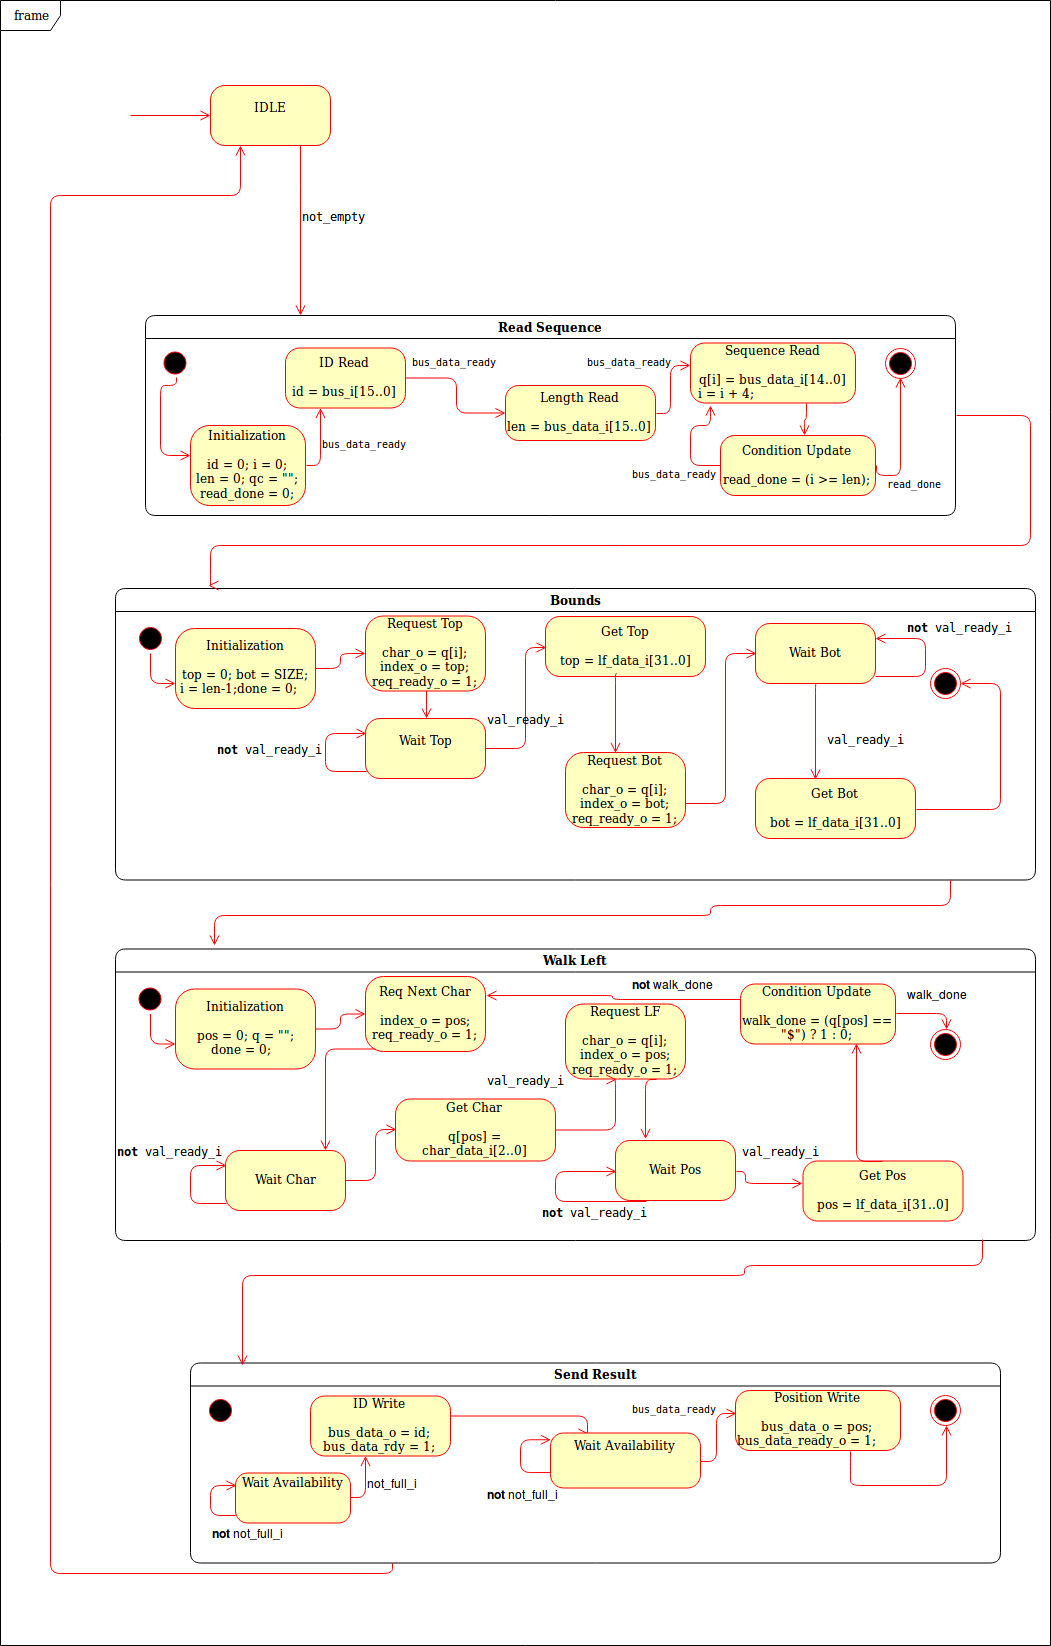
\includegraphics[scale = 0.4]{Figures/MSS.png}
    \caption{Global view of the FM-Index FSM}
    \label{fig:fsm}
\end{figure}

\subsection{ReadWrite\_Stream}

[SIMPLE SCHEMA BLOCK, FSM]

This block is responsible for reading the received data by the streaming bus. Those data start by the \textsl{short read} ID and size, followed by the actual sequence, already encoded and inverted. The first information are stored in registers and the short read itself is placed into a buffer : once a line is ready, the global FSM is notified, and the reading continue.

\subsection{Bounds}

[SIMPLE SCHEMA BLOCK, FSM] \\


 This block reads this sequence from the buffer on line at a time, once all elements from it have been used, it notifies the upper level it is ready for the next one and continues until it has read \textrm{size} elements. For each read symbol iteration, the top and bottom position outputs are updated one after the other. After each update, both the number of read symbol and the new positions are evaluated and just like in Algorithm \ref{alg:match}, if at some point the interval $ [ top,bottom ] $ is empty, the loop is terminated the FSM goes back to waiting for a new sequence.

\subsection{Walk-Left}

[SIMPLE SCHEMA BLOCK, FSM] \\

Upon termination of the \textsl{Bounds} algorithm, this block is notified that a new data is available. At the present time, only the \textsl{top} position is used. Hence, only one match - given there are at least one - is returned for each provided short read. As presented in Algorithm \ref{alg:WL}, this block first checks if there is a Suffix-Array index sample available for the provided position. If that's the case, it queries this value to the memory and returns it directly. If not, it fetches the BWT symbol corresponding to the current position and update this position using said symbol and said position for a LF-Mapping, and increments the number of step done so far. Then again, the new position is evaluated for a Suffix-Array index sample and so on and so forth until either the current position has such a sample, or the termination symbol \"\#\" is reached.
In the first case, the returned position is the number of step added to the index sample, in the latter, the number of steps is returned. \\

In both cases, the returned position corresponds to the short read position in the original (untransformed) text \textsl{T}.

\subsection{Last-First}

[SIMPLE SCHEMA BLOCK, FSM] \\

This block, used by both the \textsl{Bounds} and \textsl{Walk\_Left} blocks is the central processing unit of the FM-Index. This bloc aims to implement the mapping between the \textsl{BWT} symbols and their respective index in the conceptual suffix array first column (Equation \ref{eq:LF}. For each symbol of \textsl{T's} alphabet, its \textsl{Occ} value can be provided via a dedicated interface and placed into local registers. In order to determine the \textsl{Count} value of the provided inputs, it first queries the closest checkpoint value corresponding to the given symbol. It then iteratively queries \textsl{BWT} symbol from this position until it reaches the given position, incrementing a local count value each time the obtained symbol corresponds to the input.

Upon termination, the sum of all three values is returned. \\

Considering this methods of implementing \textsl{LF} requires querying symbols from the BWT, this block also provides this function to the rest of the system (only used by \textsl{Walk\_Left}, hence the input signal \textrm{getChar\_nLF\_i} that indicates which operation is demanded. To this end, an output signal \textrm{sbl\_o} is used to return the obtained symbol upon request.

\section{VHDL Implementation}

Mettre ici la figure d'avant, changer la figure d'avant pour enlever tous les trucs RTL : BRAM, REG, MUX et mettre juste des décideurs à la place.

Mettre RTL ?

\subsection{FMIndex}

\subsection{Read PCI}

\subsection{Last-First}

\subsection{Bounds}

\subsection{Walk-Left}



\section{Test \& Validation}

In order to validate the behavior of the whole system while keeping good handle of its complexity, a testbench suite has been developped for each bloc composing the system, with a final one for the whole \textsl{FM-Index} bloc. \\

\subsection{References}
To simulate the memory, a reference dataset has been created using the previously introduced software. Using a reference text of length 1000, all the elements have been computed and place in reference files :

\begin{description}
\item [bwt\_pkg -] This file contains an array of all the BWT symbols in correct orders
\item [ssa\_pkg -] This file contains an array of all the sampled Suffix-Array indices
\item [chkX\_pkg -] Those files, one for each symbol A, C, G, T, and N contains an array of all the sampled checkpoints for each of those.
\item [lfX\_pkg -] Like the previous files, each one of those contains a lookup-table of Eq. \ref{eq:LF} for each possible entry.
\end{description}

\subsection{Global Structure}

\begin{figure}[H]
 \includegraphics[scale = 0.4]{Figures/}
    \caption{Global view of the FM-Index FSM}
    \label{fig:fsm}
\end{figure}

Each testbench is defined according to the same structure, as depicted in Figure \ref{fig:Tb_struct}. For each DUT, a record is defined for each input sender and output receiver






